\section{recordtablemodel Class Reference}
\label{classrecordtablemodel}\index{recordtablemodel@{recordtablemodel}}
{\tt \#include $<$recordtablemodel.h$>$}

Collaboration diagram for recordtablemodel:\begin{figure}[H]
\begin{center}
\leavevmode
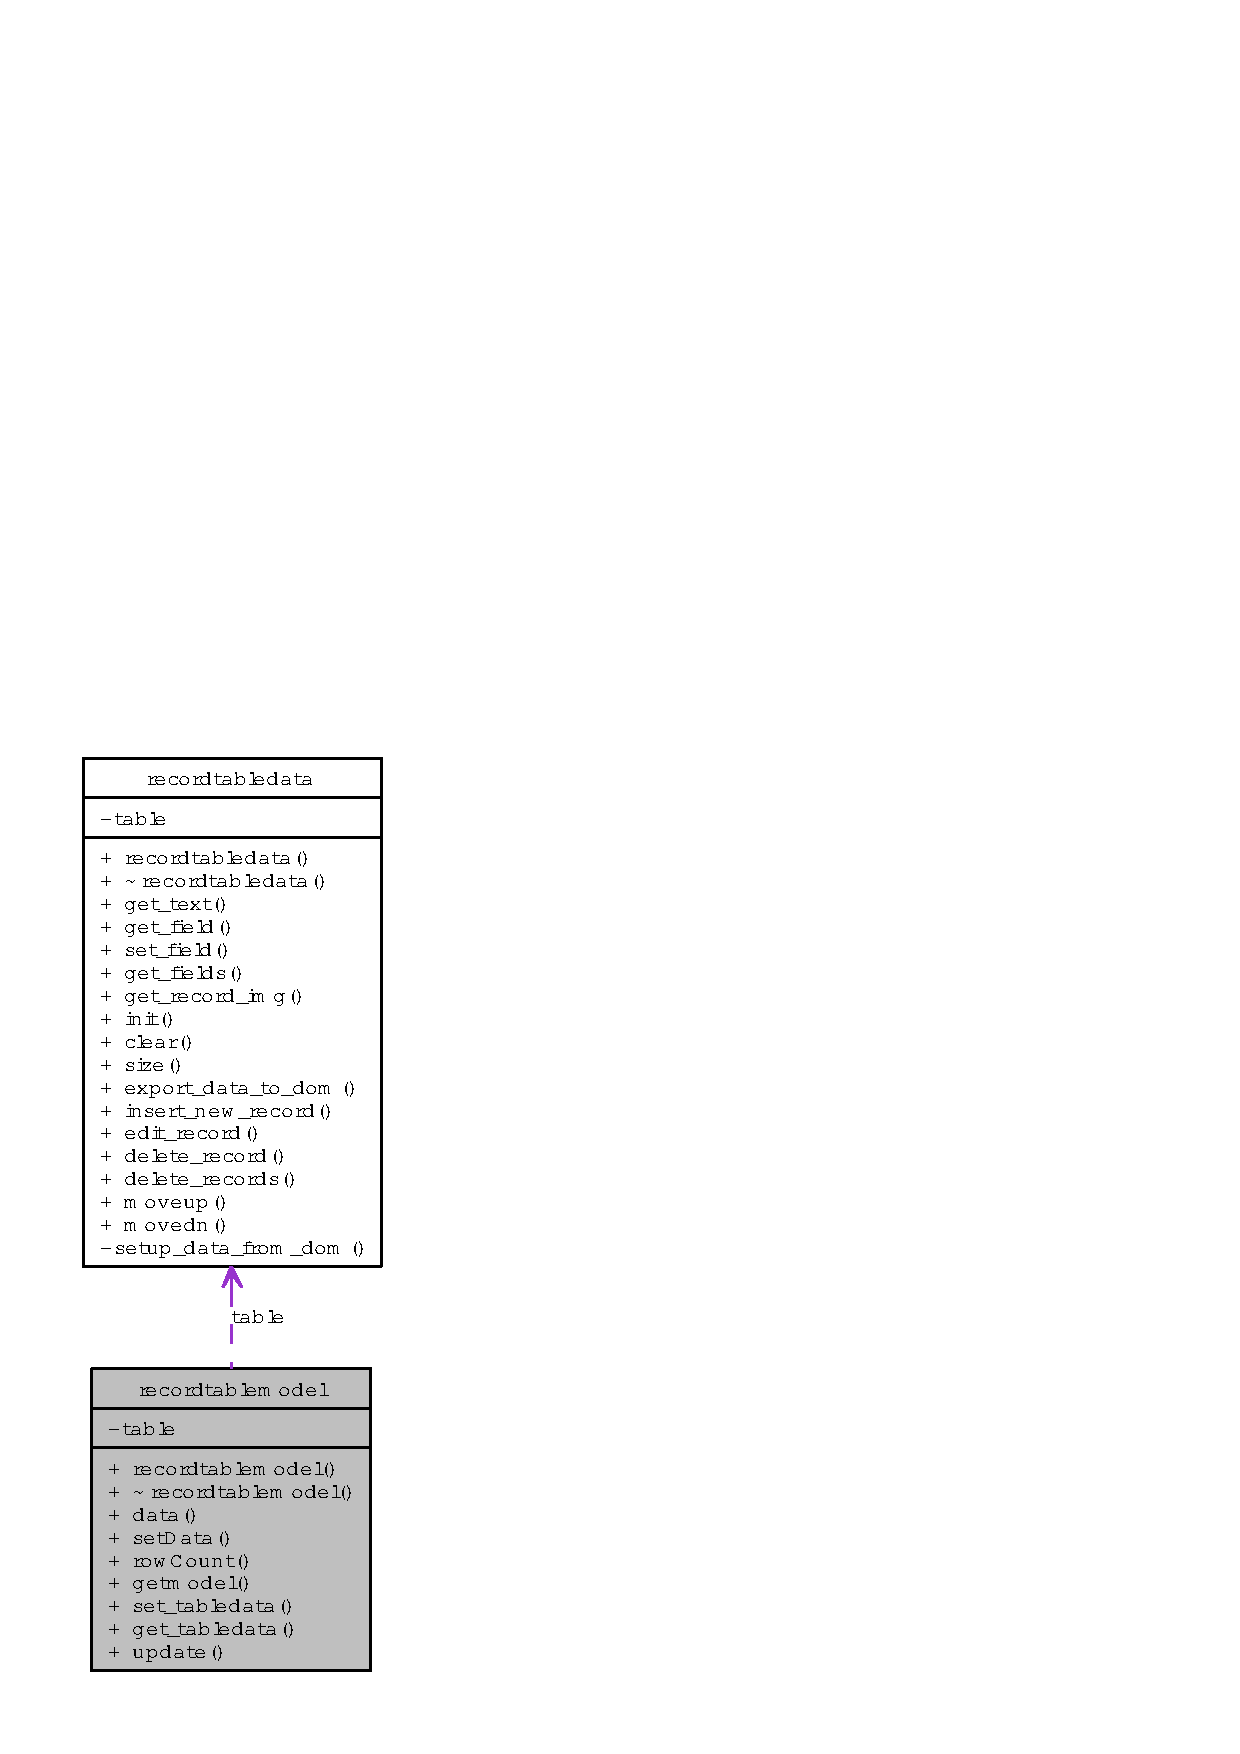
\includegraphics[width=93pt]{classrecordtablemodel__coll__graph}
\end{center}
\end{figure}
\subsection*{Public Member Functions}
\begin{CompactItemize}
\item 
{\bf recordtablemodel} (QObject $\ast$pobj=0)
\item 
{\bf $\sim$recordtablemodel} ()
\item 
QVariant {\bf data} (const QModel\-Index \&index, int n\-Role) const
\item 
bool {\bf set\-Data} (const QModel\-Index \&index, const QVariant \&value, int n\-Role)
\item 
int {\bf row\-Count} (const QModel\-Index \&parent=QModel\-Index()) const
\item 
QAbstract\-List\-Model $\ast$ {\bf getmodel} (void)
\item 
void {\bf set\_\-tabledata} ({\bf recordtabledata} $\ast$rtdata)
\item 
{\bf recordtabledata} $\ast$ {\bf get\_\-tabledata} (void)
\item 
void {\bf update} (void)
\end{CompactItemize}
\subsection*{Private Attributes}
\begin{CompactItemize}
\item 
{\bf recordtabledata} $\ast$ {\bf table}
\end{CompactItemize}


\subsection{Detailed Description}




Definition at line 13 of file recordtablemodel.h.

\subsection{Constructor \& Destructor Documentation}
\index{recordtablemodel@{recordtablemodel}!recordtablemodel@{recordtablemodel}}
\index{recordtablemodel@{recordtablemodel}!recordtablemodel@{recordtablemodel}}
\subsubsection{\setlength{\rightskip}{0pt plus 5cm}recordtablemodel::recordtablemodel (QObject $\ast$ {\em pobj} = {\tt 0})}\label{classrecordtablemodel_af0c25137468c24be205b42cb34baae4}




Definition at line 15 of file recordtablemodel.cpp.

References table.\index{recordtablemodel@{recordtablemodel}!~recordtablemodel@{$\sim$recordtablemodel}}
\index{~recordtablemodel@{$\sim$recordtablemodel}!recordtablemodel@{recordtablemodel}}
\subsubsection{\setlength{\rightskip}{0pt plus 5cm}recordtablemodel::$\sim$recordtablemodel ()}\label{classrecordtablemodel_83350f16ce086e94a8e122801dde199f}




Definition at line 26 of file recordtablemodel.cpp.

\subsection{Member Function Documentation}
\index{recordtablemodel@{recordtablemodel}!data@{data}}
\index{data@{data}!recordtablemodel@{recordtablemodel}}
\subsubsection{\setlength{\rightskip}{0pt plus 5cm}QVariant recordtablemodel::data (const QModel\-Index \& {\em index}, int {\em n\-Role}) const}\label{classrecordtablemodel_c4715776ac34d46f44616ea560b80517}




Definition at line 34 of file recordtablemodel.cpp.

References recordtabledata::get\_\-field(), and table.

Here is the call graph for this function:\begin{figure}[H]
\begin{center}
\leavevmode
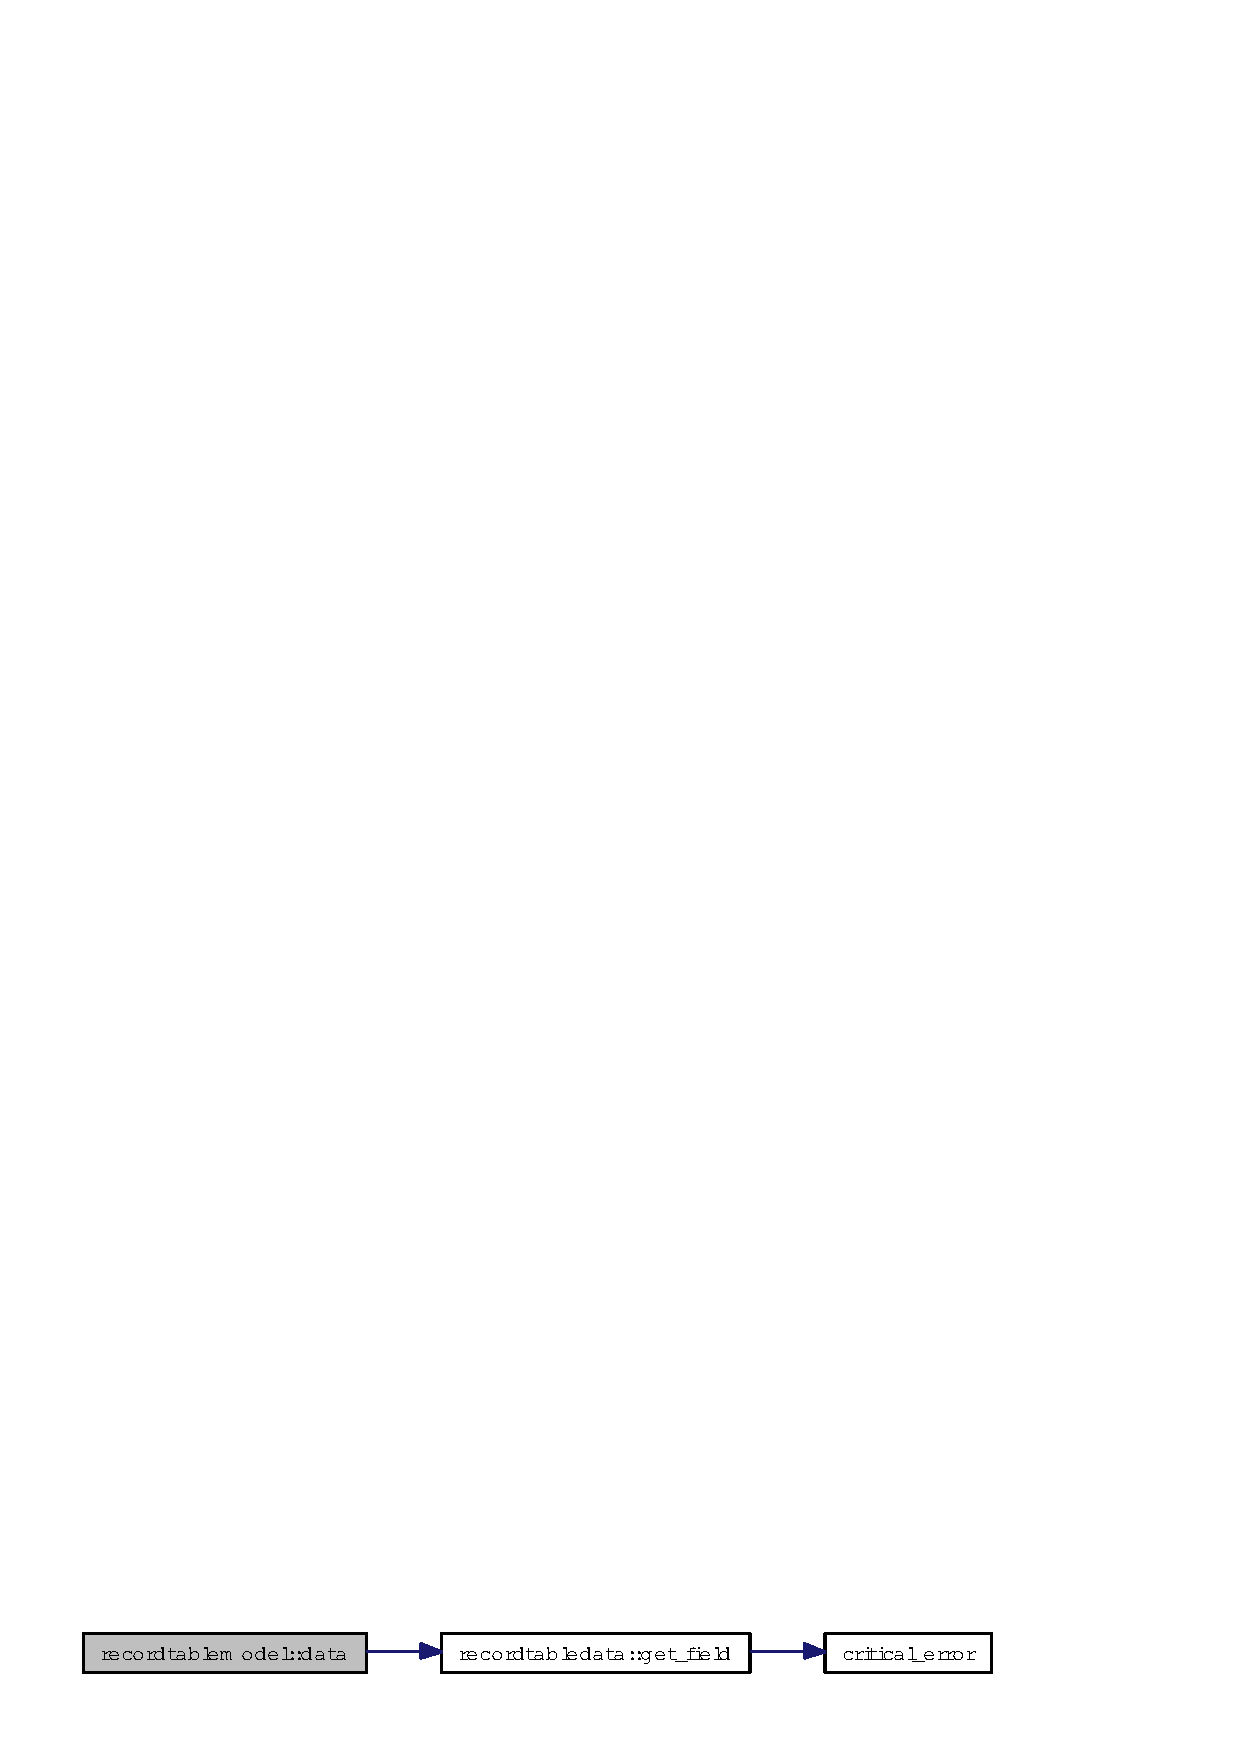
\includegraphics[width=240pt]{classrecordtablemodel_c4715776ac34d46f44616ea560b80517_cgraph}
\end{center}
\end{figure}
\index{recordtablemodel@{recordtablemodel}!setData@{setData}}
\index{setData@{setData}!recordtablemodel@{recordtablemodel}}
\subsubsection{\setlength{\rightskip}{0pt plus 5cm}bool recordtablemodel::set\-Data (const QModel\-Index \& {\em index}, const QVariant \& {\em value}, int {\em n\-Role})}\label{classrecordtablemodel_0ea466e17727cc559221747bebb052c5}




Definition at line 49 of file recordtablemodel.cpp.

References recordtabledata::set\_\-field(), and table.

Here is the call graph for this function:\begin{figure}[H]
\begin{center}
\leavevmode
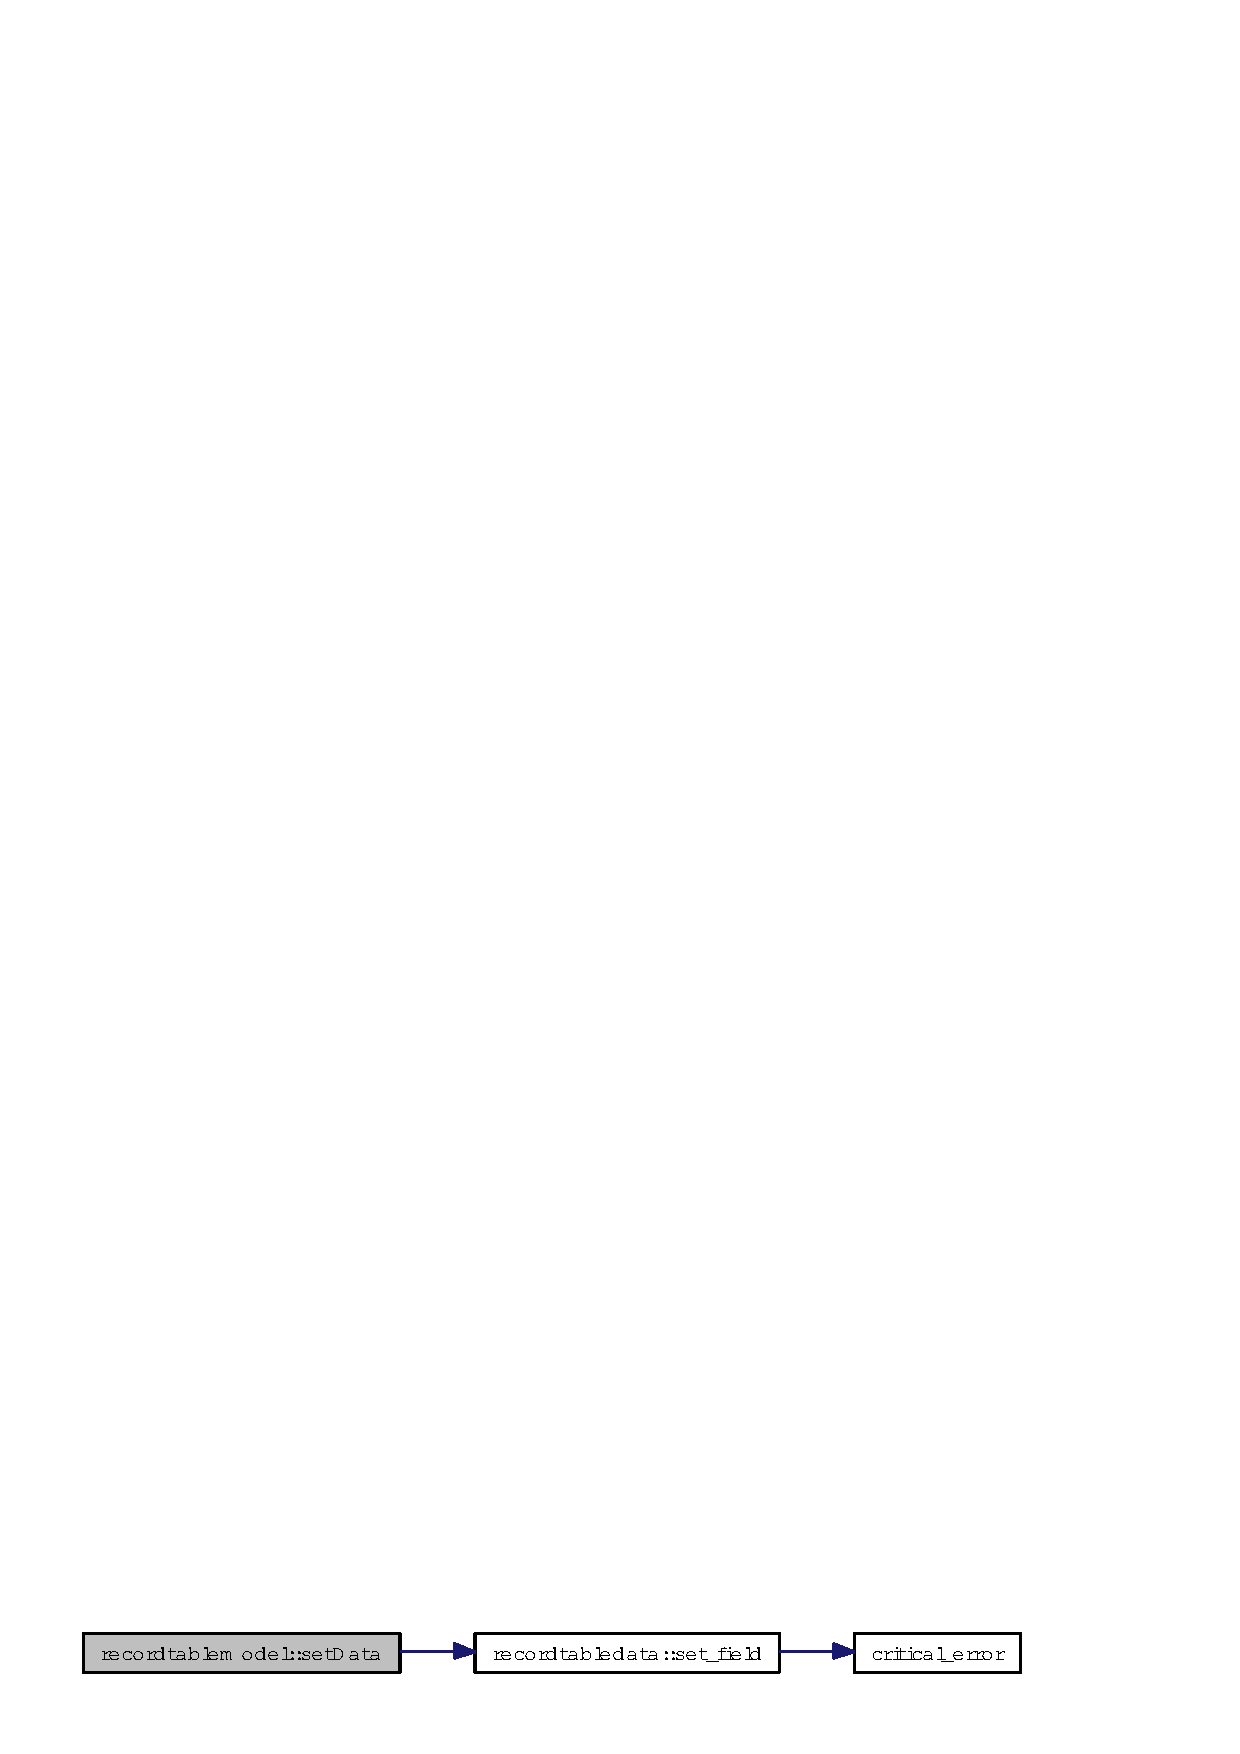
\includegraphics[width=247pt]{classrecordtablemodel_0ea466e17727cc559221747bebb052c5_cgraph}
\end{center}
\end{figure}
\index{recordtablemodel@{recordtablemodel}!rowCount@{rowCount}}
\index{rowCount@{rowCount}!recordtablemodel@{recordtablemodel}}
\subsubsection{\setlength{\rightskip}{0pt plus 5cm}int recordtablemodel::row\-Count (const QModel\-Index \& {\em parent} = {\tt QModelIndex()}) const}\label{classrecordtablemodel_d243937a7c319b06445655687347bfa0}




Definition at line 75 of file recordtablemodel.cpp.

References recordtabledata::size(), and table.

Referenced by recordtablescreen::set\_\-tabledata().

Here is the call graph for this function:\begin{figure}[H]
\begin{center}
\leavevmode
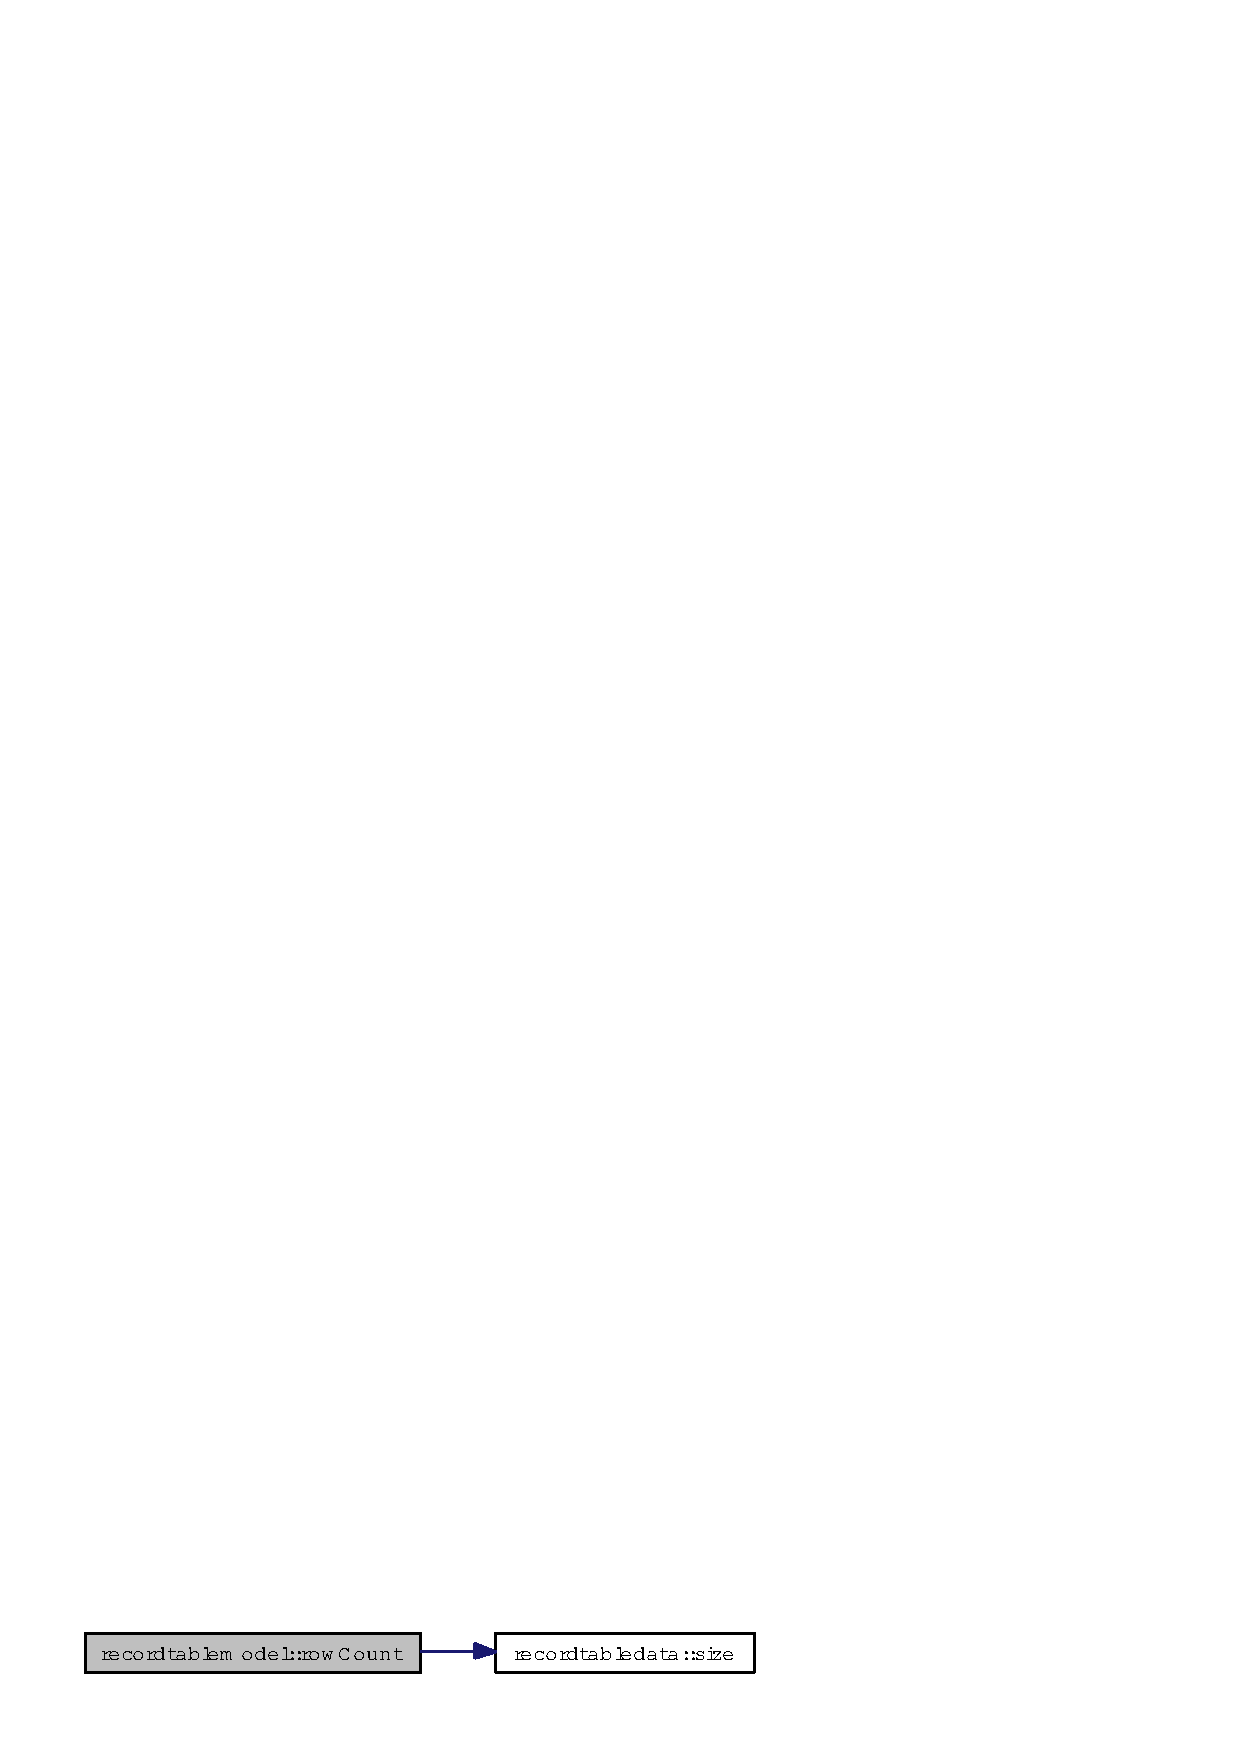
\includegraphics[width=183pt]{classrecordtablemodel_d243937a7c319b06445655687347bfa0_cgraph}
\end{center}
\end{figure}


Here is the caller graph for this function:\begin{figure}[H]
\begin{center}
\leavevmode
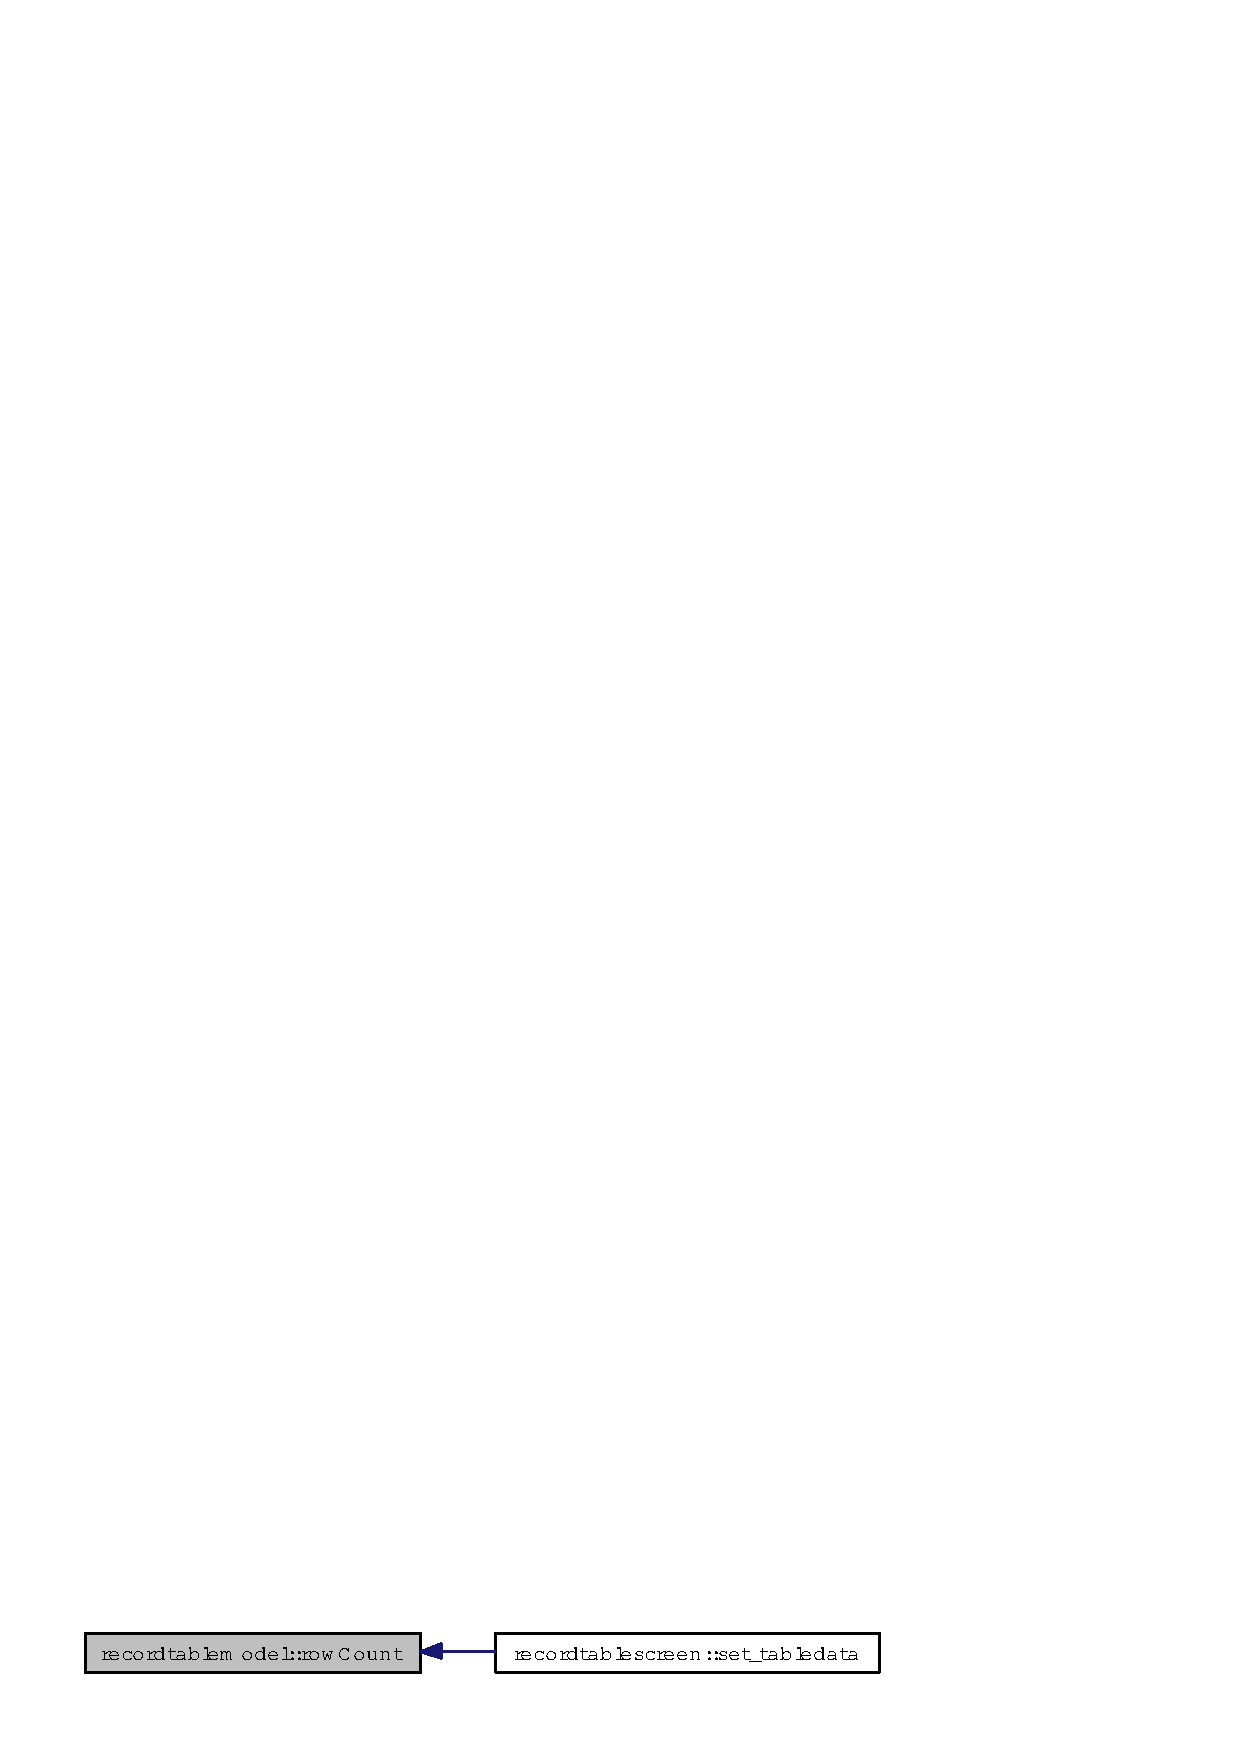
\includegraphics[width=213pt]{classrecordtablemodel_d243937a7c319b06445655687347bfa0_icgraph}
\end{center}
\end{figure}
\index{recordtablemodel@{recordtablemodel}!getmodel@{getmodel}}
\index{getmodel@{getmodel}!recordtablemodel@{recordtablemodel}}
\subsubsection{\setlength{\rightskip}{0pt plus 5cm}QAbstract\-List\-Model $\ast$ recordtablemodel::getmodel (void)}\label{classrecordtablemodel_535d23269d91adde52e73d701f84c4d3}




Definition at line 82 of file recordtablemodel.cpp.\index{recordtablemodel@{recordtablemodel}!set_tabledata@{set\_\-tabledata}}
\index{set_tabledata@{set\_\-tabledata}!recordtablemodel@{recordtablemodel}}
\subsubsection{\setlength{\rightskip}{0pt plus 5cm}void recordtablemodel::set\_\-tabledata ({\bf recordtabledata} $\ast$ {\em rtdata})}\label{classrecordtablemodel_c7525d3fce71b4ad225169190141088f}




Definition at line 88 of file recordtablemodel.cpp.

References table.

Referenced by recordtablescreen::set\_\-tabledata().

Here is the caller graph for this function:\begin{figure}[H]
\begin{center}
\leavevmode
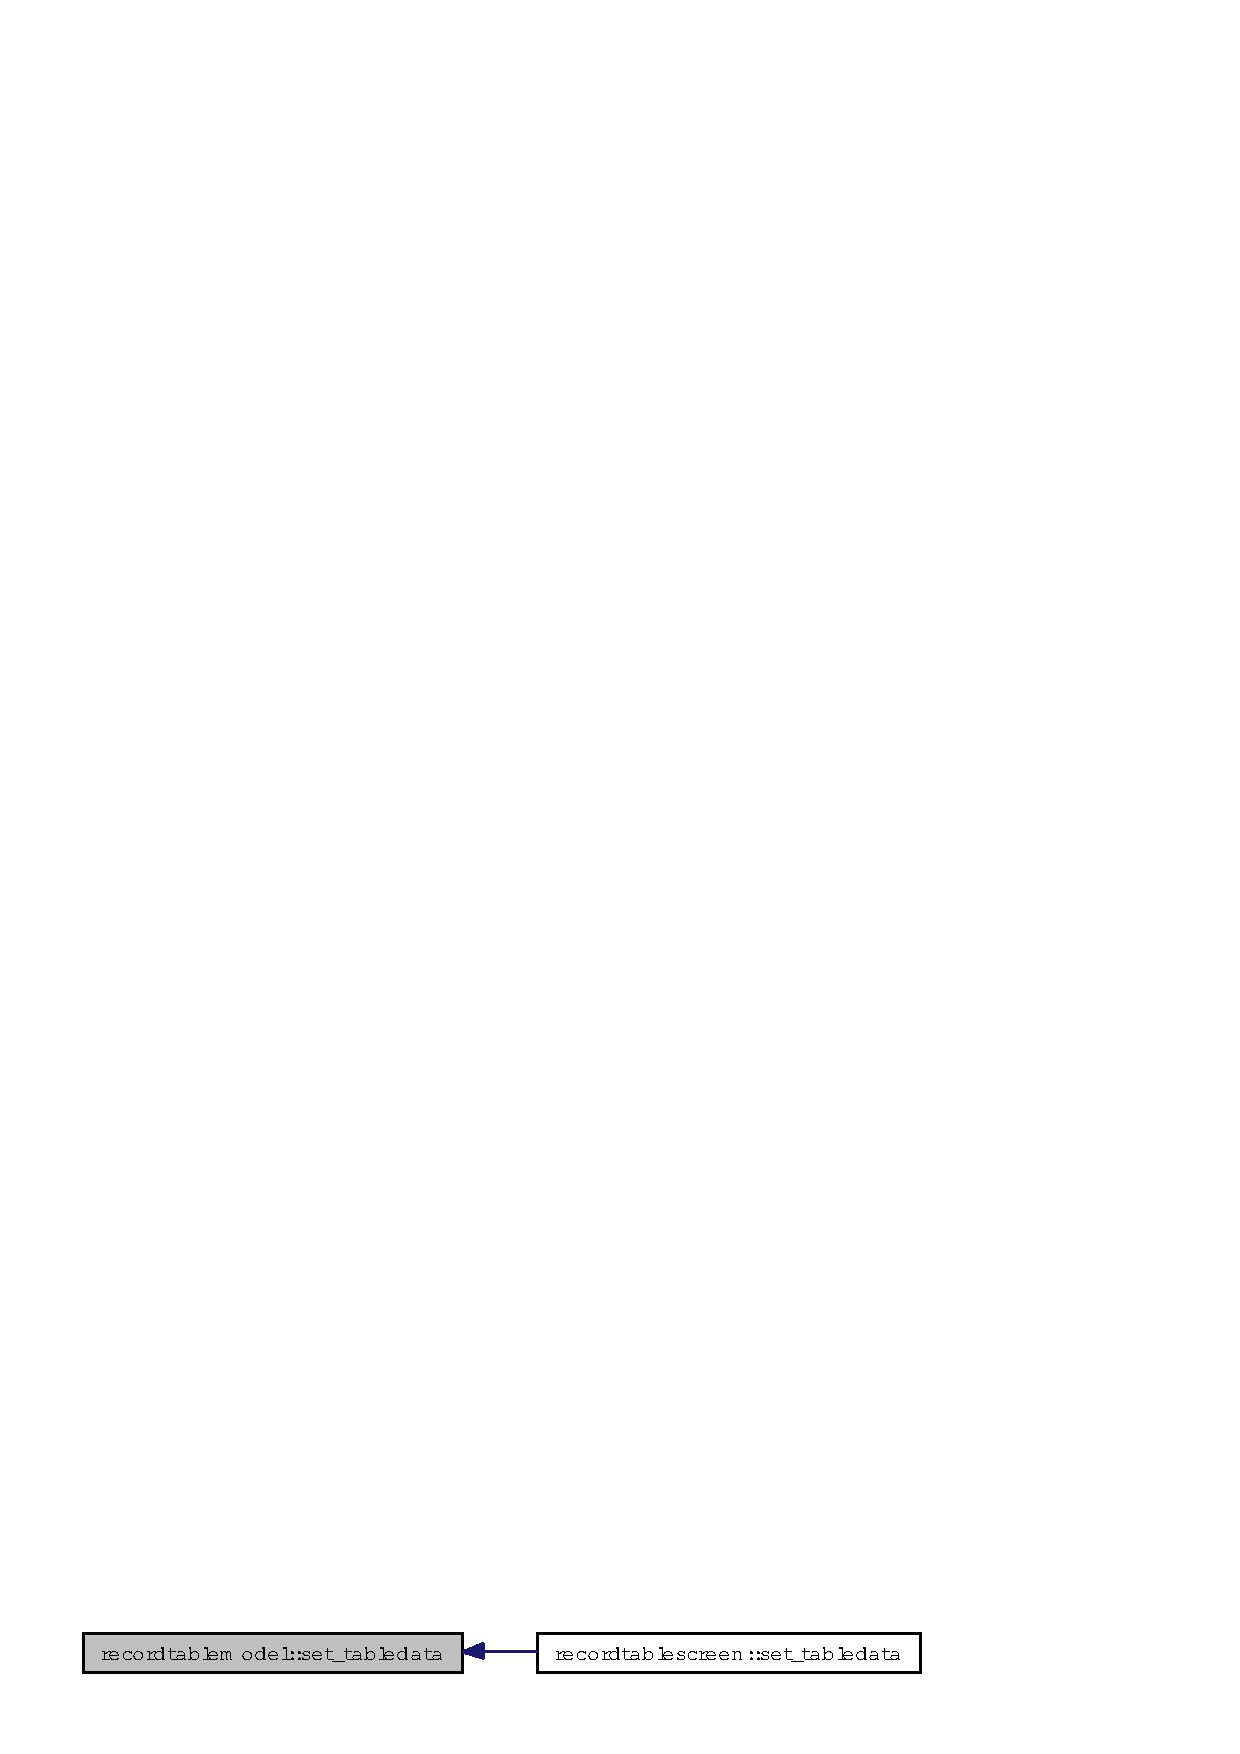
\includegraphics[width=223pt]{classrecordtablemodel_c7525d3fce71b4ad225169190141088f_icgraph}
\end{center}
\end{figure}
\index{recordtablemodel@{recordtablemodel}!get_tabledata@{get\_\-tabledata}}
\index{get_tabledata@{get\_\-tabledata}!recordtablemodel@{recordtablemodel}}
\subsubsection{\setlength{\rightskip}{0pt plus 5cm}{\bf recordtabledata} $\ast$ recordtablemodel::get\_\-tabledata (void)}\label{classrecordtablemodel_e3a0df4eed2846f73e7858e27ce3fdb6}




Definition at line 96 of file recordtablemodel.cpp.

References table.

Referenced by recordtablescreen::add\_\-new(), recordtablescreen::copy(), recordtablescreen::delete\_\-records(), recordtablescreen::edit\_\-field(), recordtablescreen::edit\_\-field\_\-context(), recordtablescreen::movedn(), recordtablescreen::moveup(), and recordtablescreen::select().

Here is the caller graph for this function:\begin{figure}[H]
\begin{center}
\leavevmode
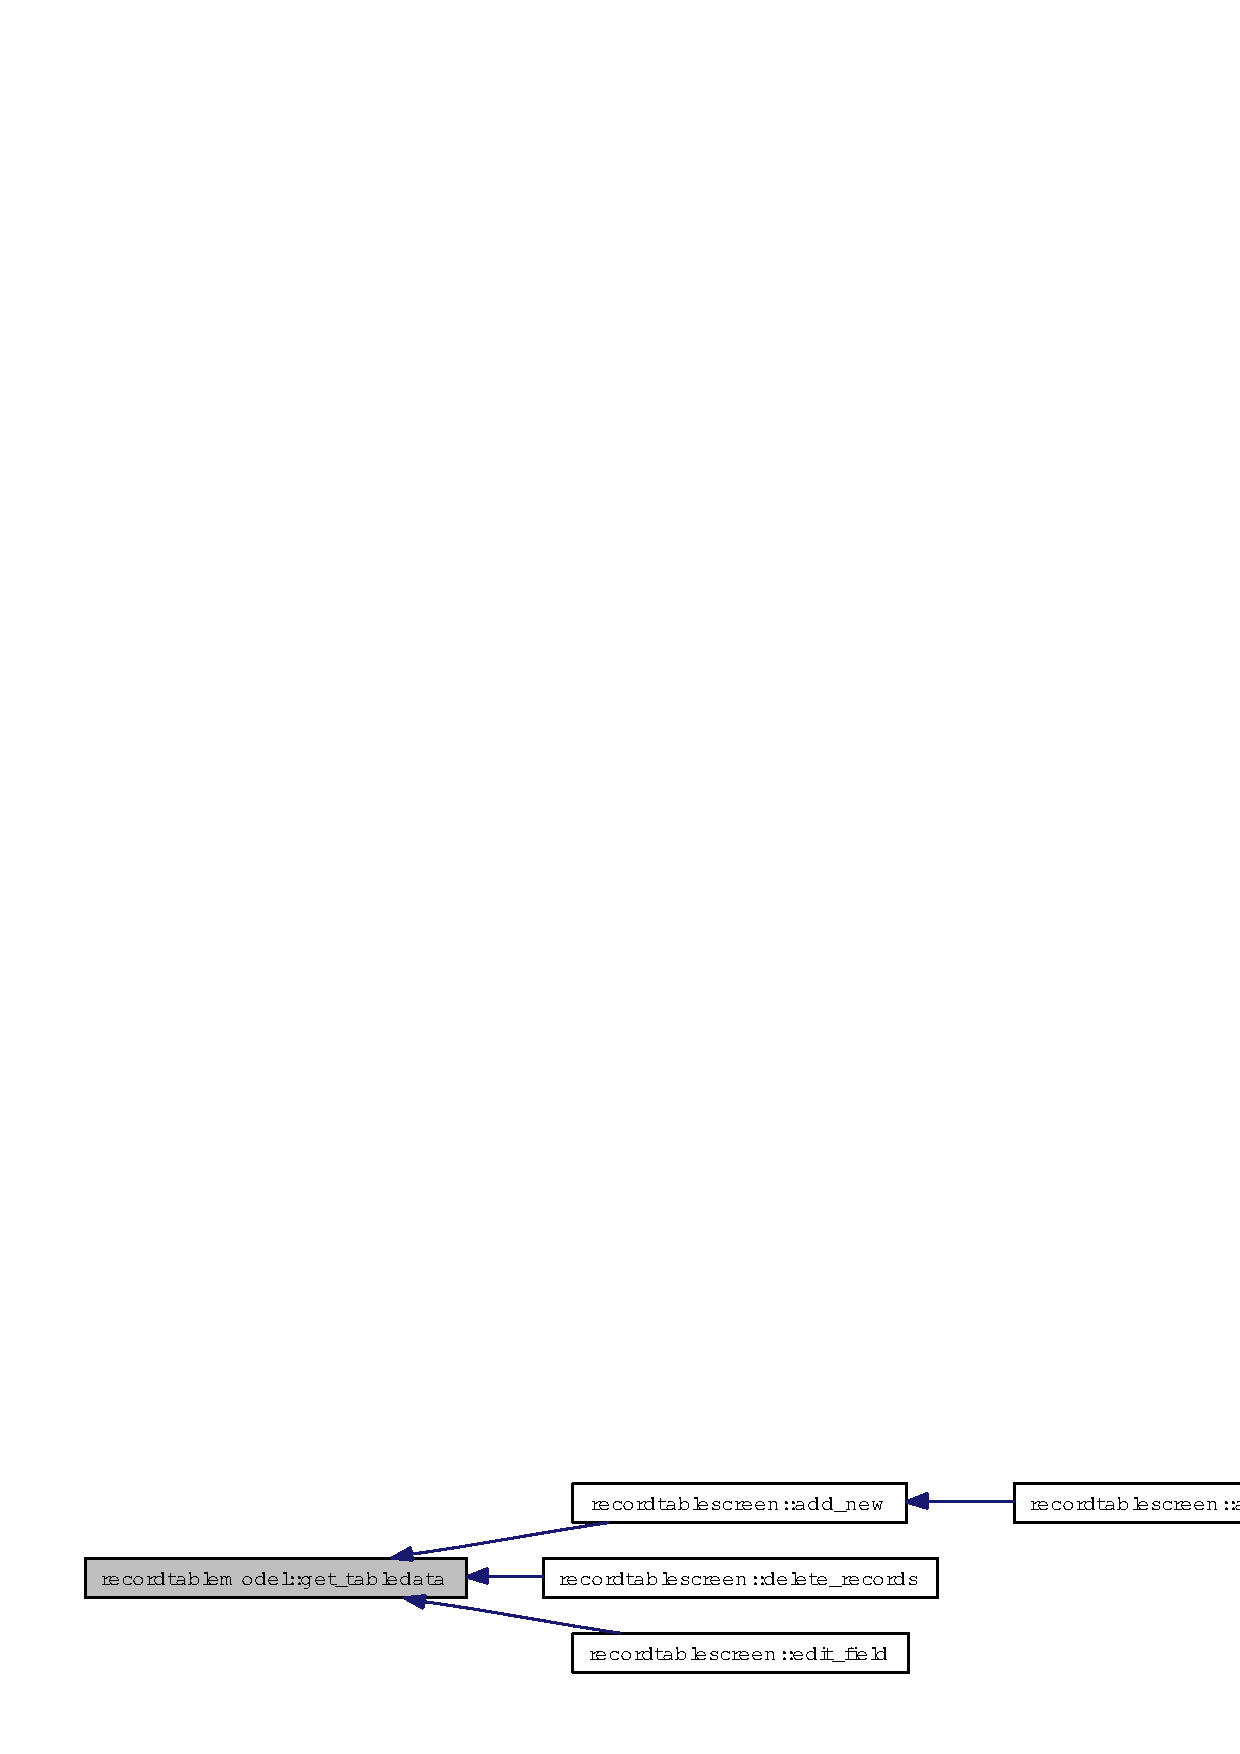
\includegraphics[width=344pt]{classrecordtablemodel_e3a0df4eed2846f73e7858e27ce3fdb6_icgraph}
\end{center}
\end{figure}
\index{recordtablemodel@{recordtablemodel}!update@{update}}
\index{update@{update}!recordtablemodel@{recordtablemodel}}
\subsubsection{\setlength{\rightskip}{0pt plus 5cm}void recordtablemodel::update (void)}\label{classrecordtablemodel_e19a2f856cd1dda4f1955af3544ce482}




Definition at line 102 of file recordtablemodel.cpp.

Referenced by recordtablescreen::add\_\-new(), and recordtablescreen::delete\_\-records().

Here is the caller graph for this function:\begin{figure}[H]
\begin{center}
\leavevmode
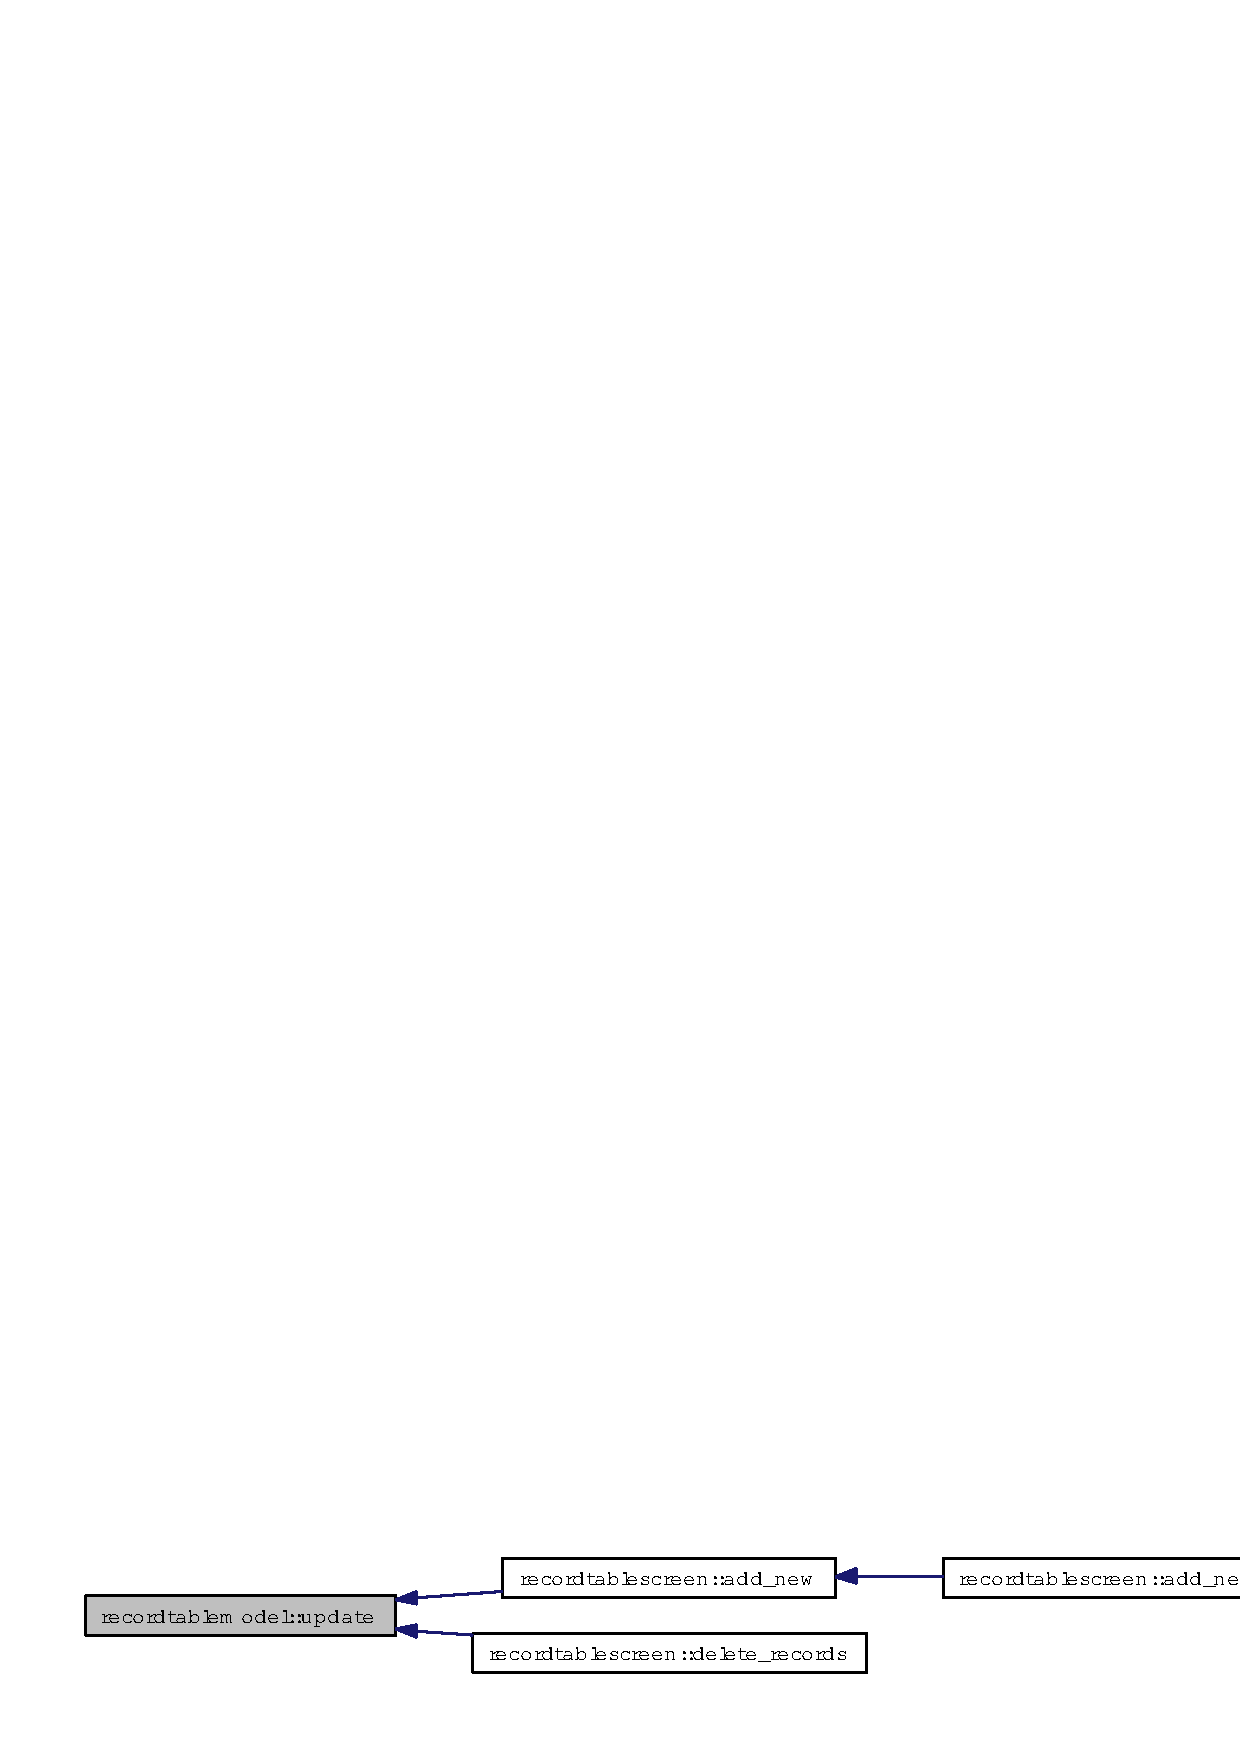
\includegraphics[width=327pt]{classrecordtablemodel_e19a2f856cd1dda4f1955af3544ce482_icgraph}
\end{center}
\end{figure}


\subsection{Member Data Documentation}
\index{recordtablemodel@{recordtablemodel}!table@{table}}
\index{table@{table}!recordtablemodel@{recordtablemodel}}
\subsubsection{\setlength{\rightskip}{0pt plus 5cm}{\bf recordtabledata}$\ast$ {\bf recordtablemodel::table}\hspace{0.3cm}{\tt  [private]}}\label{classrecordtablemodel_e8ab912d7b127a5feb5b9ef8128541d0}




Definition at line 46 of file recordtablemodel.h.

Referenced by data(), get\_\-tabledata(), recordtablemodel(), row\-Count(), set\_\-tabledata(), and set\-Data().

The documentation for this class was generated from the following files:\begin{CompactItemize}
\item 
{\bf recordtablemodel.h}\item 
{\bf recordtablemodel.cpp}\end{CompactItemize}
